\section{Sesión 18}

\begin{definicion}
	Sea $(X,\tau)$ un espacio métrico sea $p\in X$. Una vecindad de $p$ es cualquier conjunto $U\ni$ 
	\begin{enumerate}
		\item $p\in U$
		\item $\exists V\in \tau ni V\subseteq$ y $p\in V$. 
	\end{enumerate}
\end{definicion}

\begin{definicion}
	Sea $(X,\tau)$ un espacio topológico una sucesión sobre $X$ es cualquier función $f:\mathbb{Z}^+\to X$. 
\end{definicion}

\begin{definicion}
	Se dice que la sucesión $(x_n)$ en el espacio topológico $(X,\tau)$ converge a $p\in X$, si cada vecindad de $x$ contiene a la cola de la sucesión. 
\end{definicion}

\begin{definicion}
	Un conjunto $D$ es dirigido si existe una relación binaria $\geqslant$ sobre $D\ni$ 
	\begin{enumerate}
		\item $m\leqslant m, \forall m\in D$. 
		\item Si $m\leqslant n$ y $n\leqslant r\implies m\leqslant r$. 
		\item Si $m,n\in D\implies \exists r\in D\ni m\leqslant r$ y $n\leqslant r$. 
	\end{enumerate}
Entonces, $(D,\leqslant)$ es el conjunto dirigido y a $\leqslant$ se le llama dirección. 
\end{definicion}

\begin{definicion}
	Una \textbf{red} es un conjunto $X$ es una función $f:D\to X$, donde $D$ es un conjunto dirigido. 
\end{definicion}
\begin{enumerate}
	\item Si $D=\mathbb{Z}^+\implies$ la red es una sucesión.
	\item Notación $(X_m)_{m\in D}$. 
	\item Red es también conocida como sucesión de Moore-Smith.
\end{enumerate}


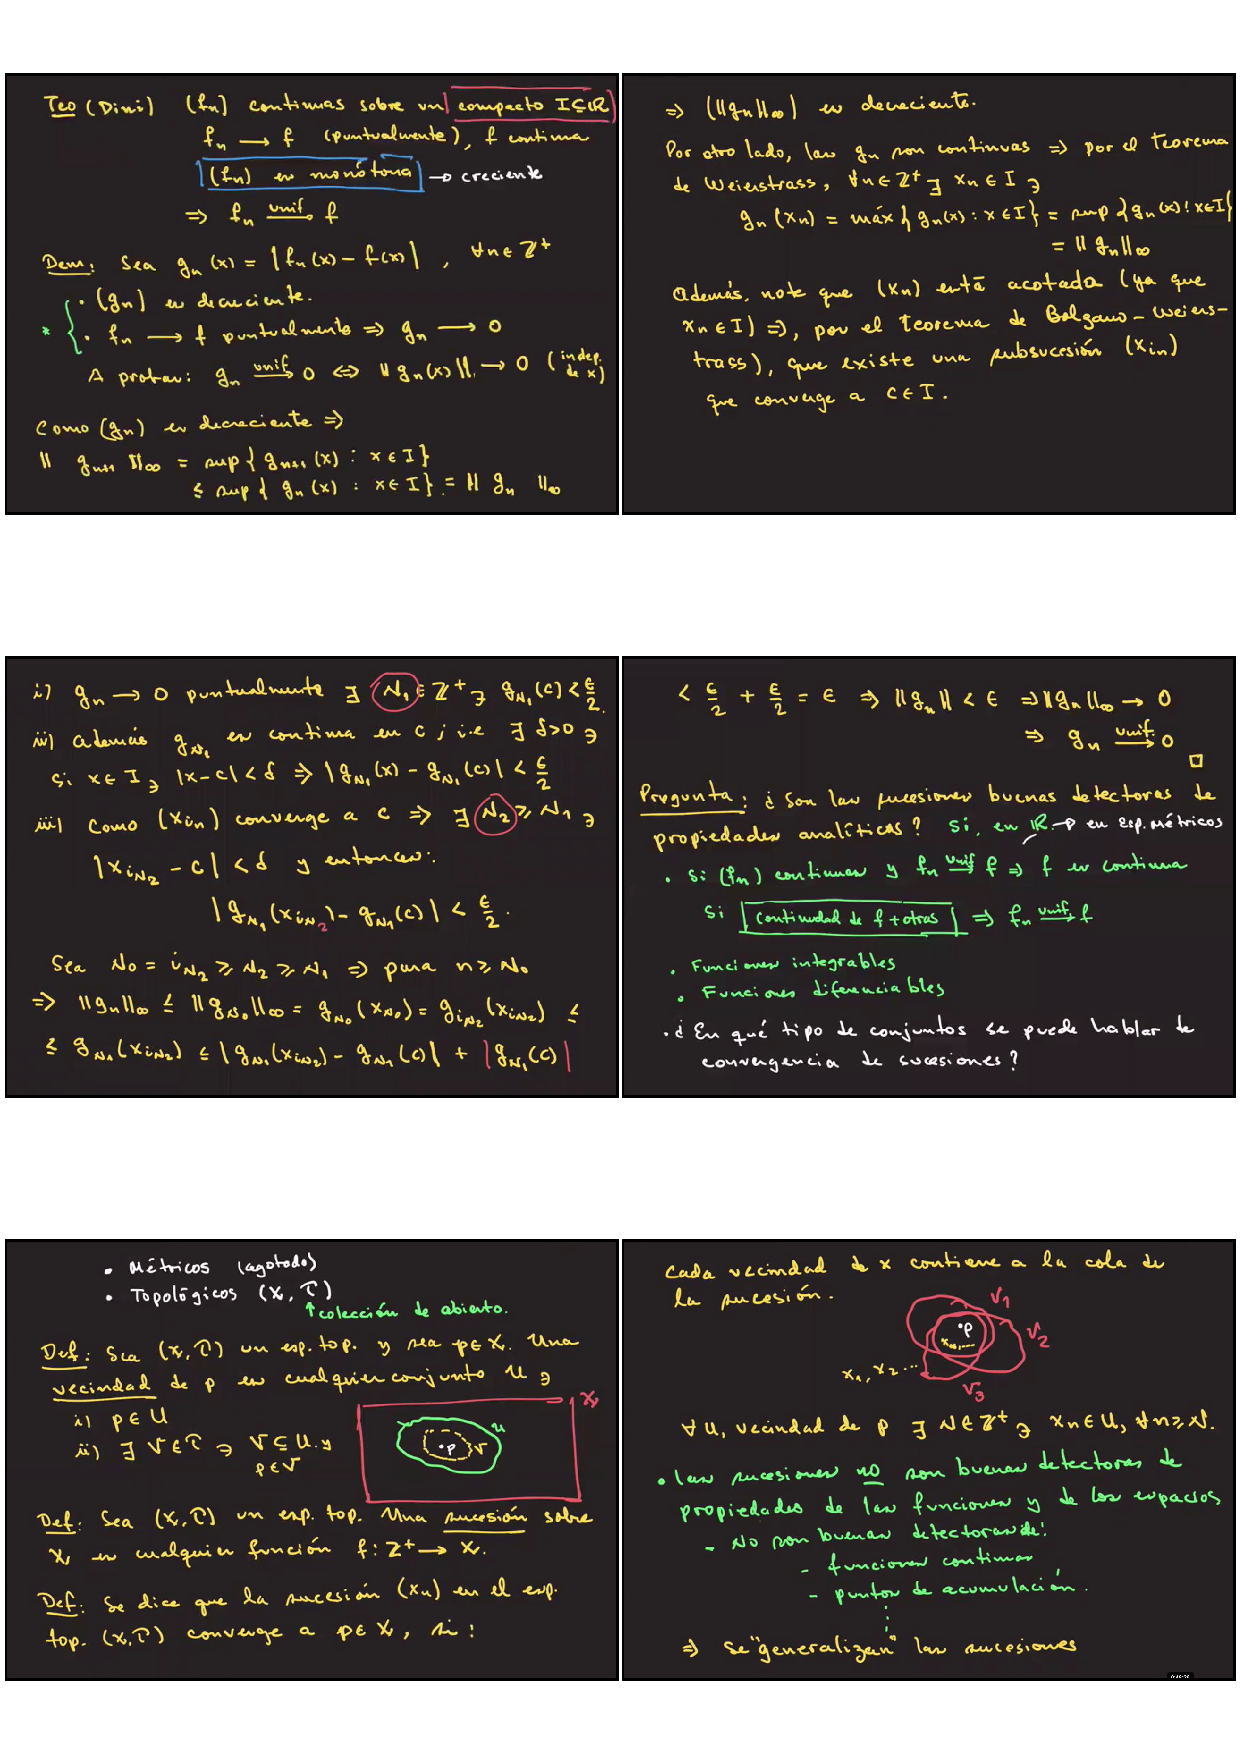
\includepdf[pages=-]{apendices/s18.pdf}